\documentclass[10pt,a4paper]{article}
\usepackage[margin=0.7in]{geometry}
\usepackage{graphicx}
\usepackage{booktabs}
\usepackage{xcolor}
\usepackage{enumitem}
\usepackage{titlesec}
\usepackage{parskip}

\titleformat{\section}{\normalsize\bfseries\color{black!80}}{}{0pt}{}
\titlespacing*{\section}{0pt}{18pt}{6pt}
\setlength{\parskip}{2pt}
\pagestyle{empty}

\begin{document}

\begin{center}
  {\large\bfseries Short-Horizon Mean-Reversion on BTCUSDT Perpetuals}\\[1pt]
  {\footnotesize Historical Performance Summary \quad$\cdot$\quad March 2026}
\end{center}

\vspace{6pt}\hrule\vspace{6pt}

\section*{1.\ Strategy}
Short-horizon \textbf{mean-reversion} strategy on the Binance \textbf{BTCUSDT perpetual future},
targeting a 5--15~minute holding period. Signals exploit microstructure features
(\textbf{order-flow imbalance}, rolling \textbf{VWAP deviation}, Bollinger / z-score reversion,
RSI, contrarian MA crossover, volume-weighted reversal) combined into a single
weighted composite.

\section*{2.\ Data}
\begin{itemize}[leftmargin=1.2em, itemsep=0pt, topsep=2pt]
  \item Tick-level trade data: \textbf{2{,}308{,}624 trades} across two UTC days
        (\textbf{2025-04-18 to 2025-04-19}).
  \item Aggregated to \textbf{1-minute OHLCV bars} with buyer/seller-initiated
        volume split (BID = buyer-initiated, ASK = seller-initiated).
\end{itemize}

\section*{3.\ Method}
Eight individual signals are computed on the bar series, each normalized to roughly
$[-1,1]$. They are combined into a weighted composite (VWAP reversion overweighted at 20\%),
smoothed with a 5-bar EMA. The smoothed composite is used directly as a continuous
position size in $[-1, +1]$.

\textbf{Execution assumptions:} positions are taken at bar close with a \textbf{1-bar
delay} (no look-ahead); PnL is captured over the subsequent bar's return. Round-trip
transaction costs are charged on every position change.

\section*{4.\ Results}

\begin{minipage}[t]{0.48\linewidth}
\vspace{0pt}
\footnotesize
\begin{tabular}{lrr}
\toprule
 & \textbf{Gross} & \textbf{Net (0.5 bps)} \\
\midrule
Total PnL (2 days)      & $+0.0300$ & $+0.0114$ \\
Annualized Sharpe       & $+43.2$   & $+16.4$   \\
Max drawdown            & $-0.0036$ & $-0.0036$ \\
Win rate                & 53\%      & 52\%      \\
Walk-forward Sharpe     & $+47.2$   & $+20.1$   \\
\bottomrule
\end{tabular}

\vspace{4pt}
{\scriptsize\hyphenpenalty=10000\exhyphenpenalty=10000\sloppy
Sharpe is annualized assuming 1-min bars
($\sqrt{1440\times 365}$ scaling). With only two days of data, point estimates
carry wide confidence intervals --- the Sharpe figures should be read as
\emph{ordinal} evidence of edge, not literal.\par}
\end{minipage}
\hfill
\begin{minipage}[t]{0.49\linewidth}
\vspace{0pt}
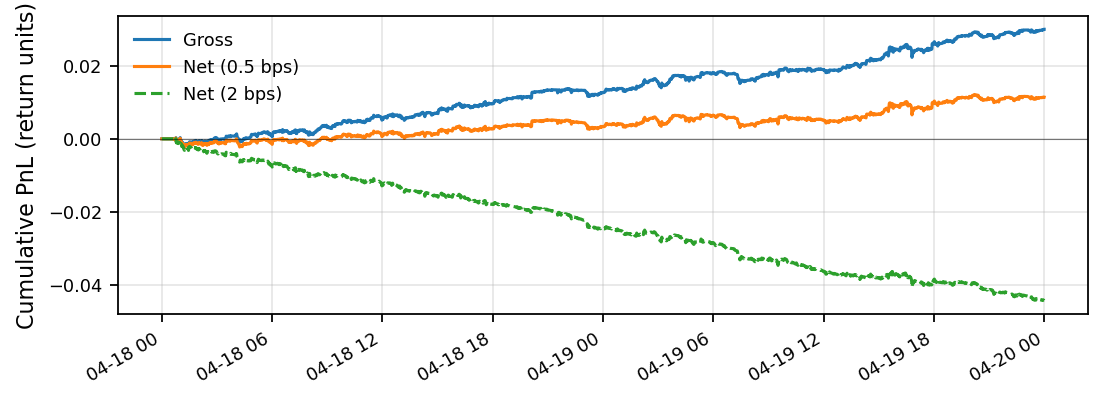
\includegraphics[width=\linewidth]{equity_curve.png}\\[-2pt]
{\scriptsize\centering Cumulative PnL: gross alpha is real but vanishes near 1\,bps.}
\end{minipage}

\section*{5.\ Cost Awareness}

\begin{tabular}{lcccccc}
\toprule
\textbf{Cost (bps round-trip)} & 0.00 & 0.25 & 0.50 & \textbf{0.75} & 1.00 & 2.00 \\
\midrule
Annualized Sharpe              & $+43.2$ & $+29.8$ & $+16.4$ & $\sim$0 & $-10.4$ & $-63.2$ \\
\bottomrule
\end{tabular}

\smallskip
\textbf{Breakeven cost is $\approx$0.75~bps round-trip.} Performance is therefore
\textbf{highly cost-sensitive}: the strategy \textbf{likely requires maker execution}
on Binance VIP tiers (where rebates can reach $-0.01$\,bps).
At a typical 2~bps taker cost, all gross alpha is consumed and the strategy is
unambiguously unprofitable.

\section*{6.\ Caveats}
Two days of data is far too short for robust inference; reported Sharpe ratios are
overstated relative to what should survive on a multi-month sample. The backtest
also assumes ideal fills at bar close --- it does not model queue priority,
slippage, or partial fills, all of which would further erode the thin
sub-bp edge. The result is best read as evidence that mean-reversion microstructure
signals are \emph{detectable} on this instrument, contingent on maker execution.

\end{document}
